\documentclass{beamer}

\usetheme{zg}
\usepackage{ulem}

\title{Orientação a Objetos}
\date{\today}
\author{Fernando Camargo}
\institute{ZG Soluções}


\begin{document}
\maketitle

\section{Por que um tema tão básico?}

\begin{frame}{Por que um tema tão básico?}
  \begin{center}
    
\includegraphics[width=0.7\textwidth]{por-que}
  \end{center}
\end{frame}

\section{Vantagens da Qualidade de Código}

\begin{frame}{Tempo gasto com código de má qualidade}
  \begin{center}
    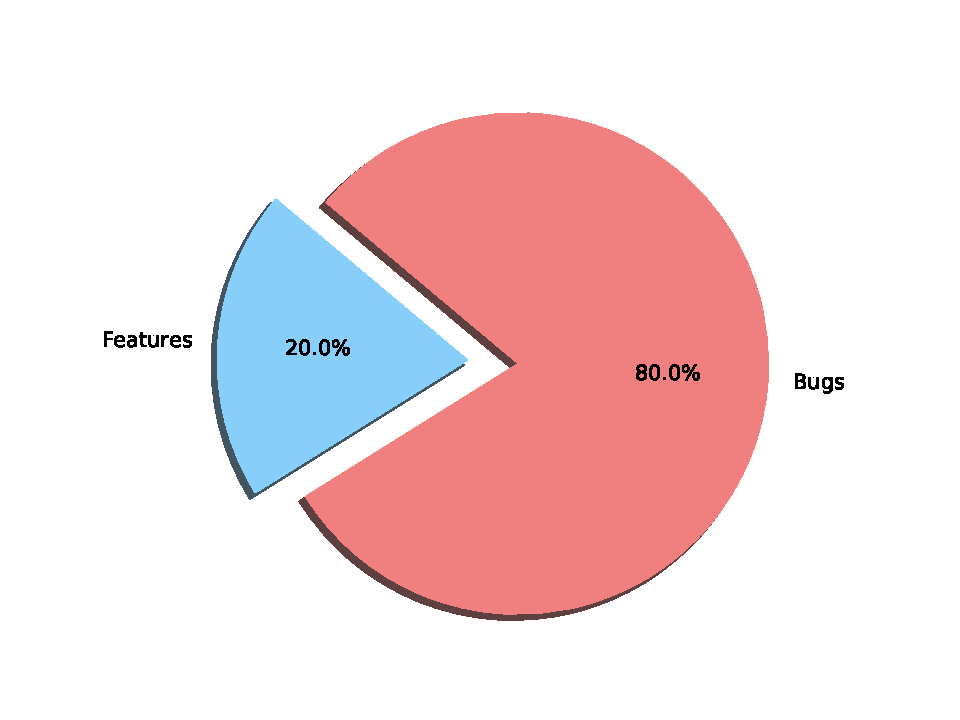
\includegraphics[width=\textwidth]{tempo-gasto-ruim}
  \end{center}
\end{frame}

\begin{frame}{Tempo gasto com código de boa qualidade}
  \begin{center}
    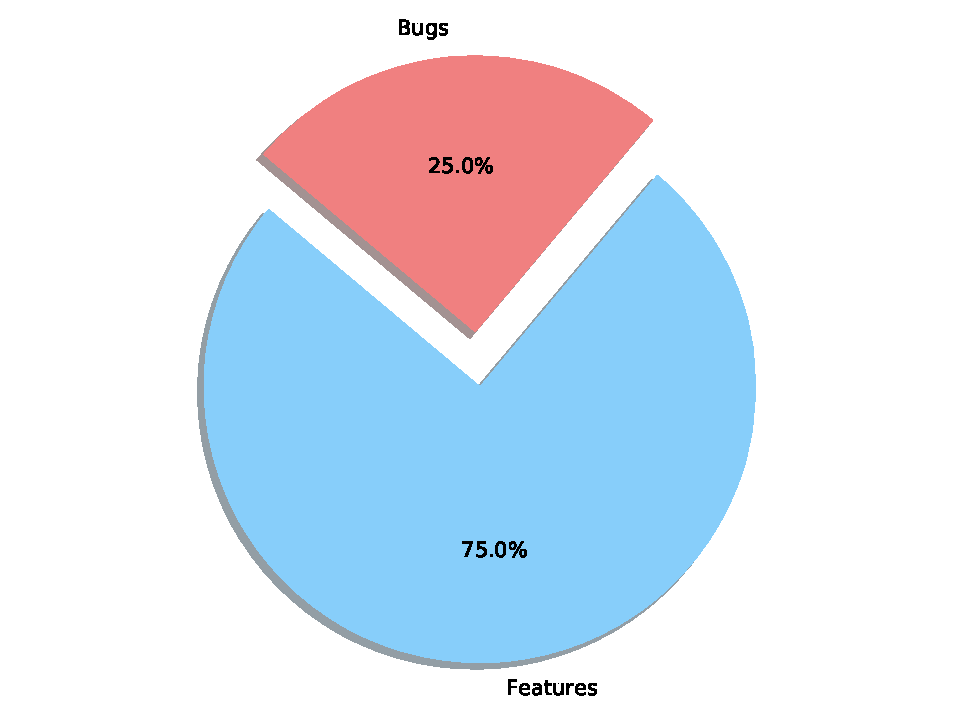
\includegraphics[width=\textwidth]{tempo-gasto-bom}
  \end{center}
\end{frame}

\section{Avaliando um Código OO}

\begin{frame}
  \begin{center}
    
\includegraphics[width=\textwidth]{todas-funcionalidades-uma-classe}
  \end{center}
\end{frame}

\subsection{Repetição de código (DRY)}

\begin{frame}{Repetição de código (DRY)}
 \begin{outline}
   \1<1-> "Don't Repeat Yourself"
   \1<2-> Lógica duplicada deve ser eliminada via abstração
 \end{outline}
\end{frame}

\subsection{Complexidade de código} % e a dificuldade de testar

\begin{frame}{Complexidade de código}
  \begin{center}
    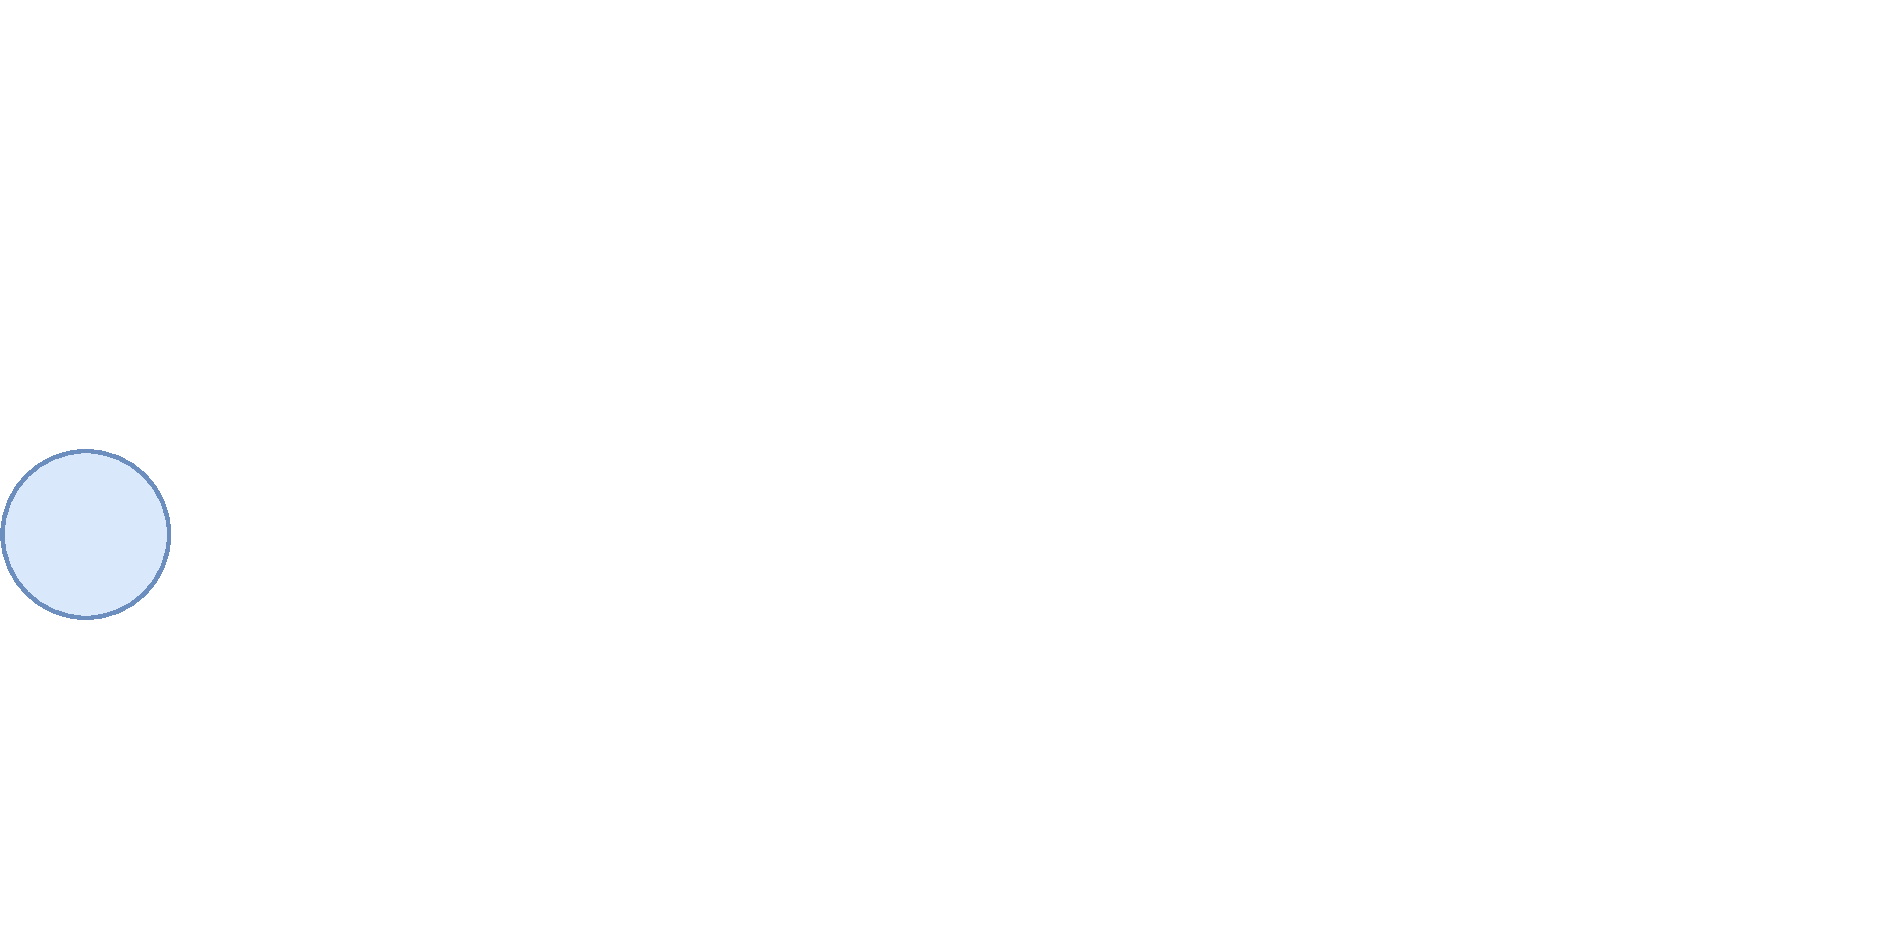
\includegraphics[width=\textwidth]{complexidade}
  \end{center}
\end{frame}

\subsection{Acoplamento} % e a alteração em cascata

\begin{frame}{Acoplamento}
  \begin{center}
    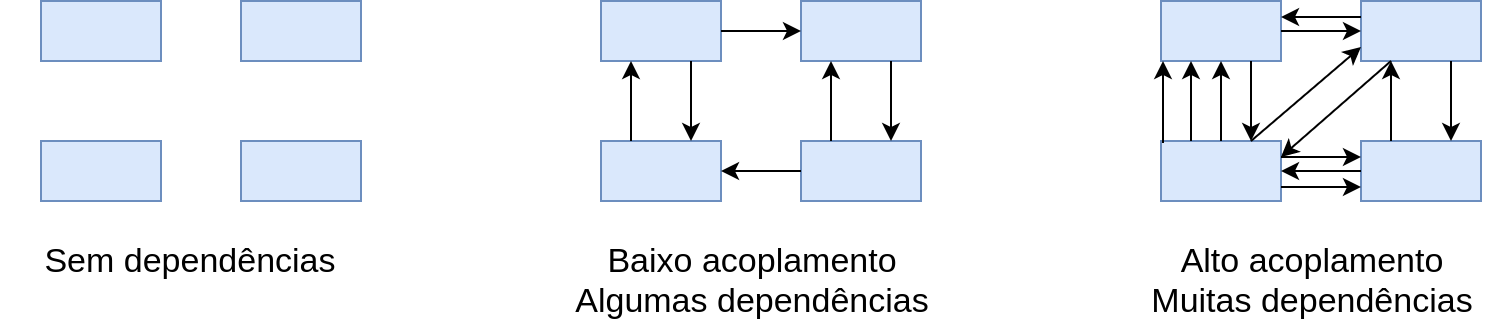
\includegraphics[width=\textwidth]{acoplamento}
  \end{center}
\end{frame}

\begin{frame}{Acoplamento}
 \begin{outline}
   \1<1-> Não existe zero acoplamento
   \1<2-> Baixo acoplamento $\rightarrow$ alterações pontuais
   \1<3-> Alto acoplamento $\rightarrow$ alterações em todo o código/em cascata
 \end{outline}
\end{frame}

\begin{frame}{O que causa alto acoplamento?}
 \begin{outline}
  \1<1-> Classes sabem \alert{demais} sobre as outras
    \2<2-> Acesso direto de propriedades
    \2<3-> Construção de dependências
    \2<4-> Uso de implementações ao invés de interfaces
  \1<5-> Falta de organização estruturada das classes (separação de camadas)
 \end{outline}
\end{frame}

\subsection{Coesão} % e os métodos que fazem tudo

\begin{frame}{Coesão}
 \begin{outline}
  \1<1-> Classes
    \2<2-> Baixa coesão $\rightarrow$ múltiplos métodos com responsabilidades/tarefas não relacionadas
    \2<3-> Alta coesão $\rightarrow$ classe possui uma única responsabilidade/tarefa, com métodos relacionados a ela
  \1<4-> Métodos
    \2<5-> Baixa coesão $\rightarrow$ método realiza várias tarefas
    \2<6-> Alta coesão $\rightarrow$ método com uma única tarefa, podendo chamar métodos que a complemente
 \end{outline}
\end{frame}

\section{Sintomas de Projeto de Classes em Degradação}

\begin{frame}{Sintomas}
 \begin{outline}
  \1<1-> Rigidez: toda mudança causa uma cascata de mudanças subsequentes em módulos dependentes
  \1<2-> Fragilidade: mudanças acarretam em quebras em muitos lugares diferentes
  \1<3-> Imobilidade: impossibilidade de reusar módulos em outros projetos
  \1<4-> Viscosidade: fácil fazer a "coisa errada" e difícil fazer a "coisa certa"
  \1<5-> Complexidade desnecessária: muitos elementos inúteis ou não utilizados (dead code)
  \1<6-> Repetição desnecessária: falta de abstração apropriada para evitar repetição de código
  \1<7-> Opacidade: código difícil de ser entendido
 \end{outline}
\end{frame}


\section{SOLID}

\subsection{Single Responsibility Principle}

\begin{frame}{Single Responsibility Principle}
  \begin{center}
    
\includegraphics[width=\textwidth]{unica-responsabilidade}
  \end{center}
\end{frame}

\begin{frame}{Single Responsibility Principle}
 "Uma classe deve ter um, e somente um, motivo para mudar."
\end{frame}

\begin{frame}{Single Responsibility Principle}
 \begin{outline}
  \1<1-> Mudanças de requisitos $\rightarrow$ mudanças nas responsabilidades
  \1<2-> Classes com múltiplas responsabilidades:
    \2<3-> Múltiplos motivos de mudança
    \2<4-> Acoplamento das responsabilidades $\rightarrow$ difícil alteração
  \1<5-> Conclusão: uma classe deve ter uma \alert{única} responsabilidade
 \end{outline}
\end{frame}

\subsection{Open/Closed Principle}

\begin{frame}{Open/Closed Principle}
  \begin{center}
    
\includegraphics[width=\textwidth]{aberto-fechado}
  \end{center}
\end{frame}

\begin{frame}{Open/Closed Principle}
 "Entidades de Software (classes, módulos, funções, etc.) devem ser abertas para extensão, mas fechadas para modificação."
\end{frame}

\begin{frame}{Open/Closed Principle}
 \begin{outline}
  \1 \only<1>{Uma mudança deve resultar em uma cascata de mudanças em classes dependentes.}\only<2->{\sout{Uma mudança deve resultar em uma cascata de mudanças em classes dependentes.}}
  \1<2-> Mudanças de requisito $\rightarrow$ adição de código novo sem alteração de código existente
  \1<3-> Como?
    \2<4-> Abstrações que permitam um grupo ilimitado de possíveis comportamentos $\rightarrow$ classes abstratas e interfaces
    \2<5-> Novos comportamentos adicionados por herança ou implementação de interface
    \2<6-> Classes dependem da abstração (fixa), não da implementação
 \end{outline}
\end{frame}

\begin{frame}{Open/Closed Principle}
  \begin{center}
    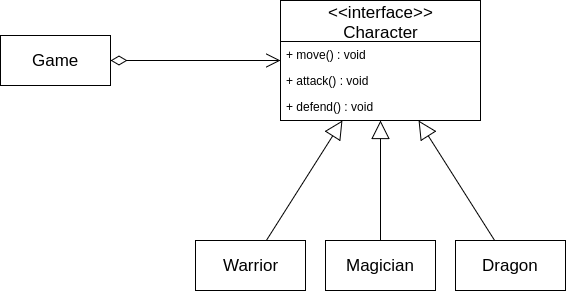
\includegraphics[width=0.9\textwidth]{diagrama-aberto-fechado}
  \end{center}
\end{frame}

\subsection{Liskov Substitution Principle}

\begin{frame}{Liskov Substitution Principle}
  \begin{center}
    
\includegraphics[width=0.7\textwidth]{substituicao}
  \end{center}
\end{frame}

\begin{frame}{Liskov Substitution Principle}
 "Uma classe base deve poder ser substituída pela sua classe derivada."
\end{frame}

\begin{frame}{Liskov Substitution Principle}
 \begin{outline}
  \1<1-> Extensão do Open/Closed Principle
  \1<2-> Classes derivadas não podem alterar o comportamento de classes base
 \end{outline}
\end{frame}

\begin{frame}[fragile]{Liskov Substitution Principle}
 \begin{minted}[fontsize=\tiny]{java}
class Square extends Rectangle {
  public void setWidth(int width){
    this.width = width;
    this.height = width;
  }

  public void setHeight(int height){
    this.width = height;
    this.height = height;
  }

}

class LspTest {
  private static Rectangle getNewRectangle() {
    return new Square();
  }

  public static void main (String args[]) {
    Rectangle r = LspTest.getNewRectangle();
        
    r.setWidth(5);
    r.setHeight(10);
    
    System.out.println(r.getArea()); // Resultado: 100 ao invés de 50
  }
}
  \end{minted}
\end{frame}

\subsection{Interface Segregation Principle}

\begin{frame}{Interface Segregation Principle}
  \begin{center}
    
\includegraphics[width=\textwidth]{opcoes}
  \end{center}
\end{frame}

\begin{frame}{Interface Segregation Principle}
 "Muitas interfaces específicas são melhores do que uma interface única."
\end{frame}

\begin{frame}{Interface Segregation Principle}
 \begin{outline}
  \1<1-> Interfaces poluídas prejudicam a coesão
  \1<2-> "Clientes não devem ser forçacos a depender de interfaces que eles não usam"
    \2<2-> Dependência de interfaces "gordas" gera acoplamento entre implementações
  \1<3-> Diferentes clientes (implementações com diferentes responsabilidades) $\rightarrow$ diferentes interfaces
 \end{outline}
\end{frame}

\begin{frame}[fragile]{ERRADO!}
 \begin{minted}[fontsize=\tiny]{java}
interface Worker {
  void work();
  void eat();
}

class FactoryWorker implements Worker {
  public void work() { /* implementation */ }
  public void eat() { /* implementation */ }
}

class Robot implements Worker {
  public void work() { /* implementation */ }
  public void eat() { /* ??? */ }
}
  \end{minted}
\end{frame}

\begin{frame}[fragile]{CORRETO!}
 \begin{minted}[fontsize=\tiny]{java}
interface Workable {
  public void work();
}

interface Feedable{
  public void eat();
}

class FactoryWorker implements Workable, Feedable {
  public void work() { /* implementation */ }
  public void eat() { /* implementation */ }
}

class Robot implements Workable {
  public void work() { /* implementation */ }
}
  \end{minted}
\end{frame}

\subsection{Dependency Inversion Principle}

\begin{frame}{Dependency Inversion Principle}
  \begin{center}
    
\includegraphics[width=0.8\textwidth]{interno}
  \end{center}
\end{frame}

\begin{frame}{Dependency Inversion Principle}
 "Dependa de uma abstração e não de uma implementação."
\end{frame}

\begin{frame}{Dependency Inversion Principle}
 \begin{outline}
  \1<1-> Implementações de baixo nível podem ser alteradas
  \1<2-> Uso dessas implementações $\rightarrow$ alto acoplamento $\rightarrow$ alterações de dependentes
  \1<3-> Uso de abstrações de alto nível (interfaces) $\rightarrow$ baixo acoplamento
 \end{outline}
\end{frame}

\begin{frame}{ERRADO!}
  \begin{center}
    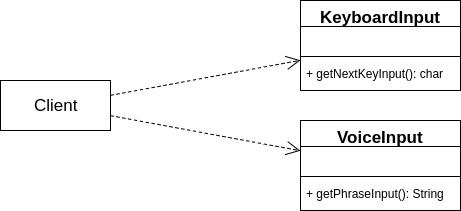
\includegraphics[width=0.9\textwidth]{diagrama-inversao-dependencia-errado}
  \end{center}
\end{frame}

\begin{frame}{CORRETO!}
  \begin{center}
    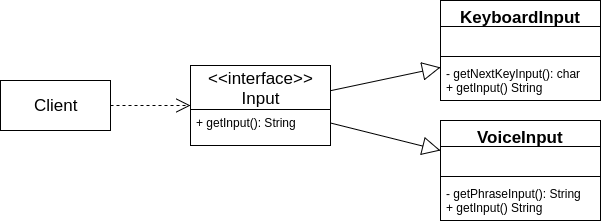
\includegraphics[width=0.9\textwidth]{diagrama-inversao-dependencia-correto}
  \end{center}
\end{frame}

\section{Conclusões}

\begin{frame}{Conclusões}
  \begin{outline}
    \1<1-> Evite \alert{repetições} de código
    \1<2-> Aplique os princípios SOLID para \alert{aumentar coesão} e \alert{reduzir acoplamento}
    \1<3-> Estude \alert{Padrões de Projeto}
  \end{outline}
\end{frame}

\end{document}